\documentclass{beamer}

%
% Common preamble for all three parts.
%

%\usepackage[english]{babel}
\usepackage[polutonikogreek, italian]{babel}
\usepackage{amsmath}
\usepackage{color}
\usepackage[cache=false]{minted}
\usepackage{hyperref}
\usepackage{multicol}
\usepackage{tabularx}
\usepackage{tikz}
\usepackage{shapepar}

% only inline todonotes work
\usepackage{xkeyval}
\usepackage[textsize=small]{todonotes}
\presetkeys{todonotes}{inline}{}

\usetikzlibrary{shapes,arrows,positioning,shadows}

% no nav buttons
\usenavigationsymbolstemplate{}

\newcommand{\bftt}[1]{\textbf{\texttt{#1}}}
\newcommand{\comment}[1]{{\color[HTML]{008080}\textit{\textbf{\texttt{#1}}}}}
\newcommand{\cmd}[1]{{\color[HTML]{008000}\bftt{#1}}}
\newcommand{\bs}{\char`\\}
\newcommand{\cmdbs}[1]{\cmd{\bs#1}}
\newcommand{\lcb}{\char '173}
\newcommand{\rcb}{\char '175}
\newcommand{\cmdbegin}[1]{\cmdbs{begin\lcb}\bftt{#1}\cmd{\rcb}}
\newcommand{\cmdend}[1]{\cmdbs{end\lcb}\bftt{#1}\cmd{\rcb}}

\newcommand{\wllogo}{\textbf{Overleaf}}

% this is where the example source files are loaded from
% do not include a trailing slash
\newcommand{\fileuri}{https://raw.github.com/mirtexxan/latex-course/master/it}

\newcommand{\wlserver}{https://www.overleaf.com}
\newcommand{\wlnewdoc}[1]{\wlserver/docs?snip\_uri=\fileuri/#1\&splash=none}

\def\tikzname{Ti\emph{k}Z}

% from http://tex.stackexchange.com/questions/5226/keyboard-font-for-latex
\newcommand*\keystroke[1]{%
  \tikz[baseline=(key.base)]
    \node[%
      draw,
      fill=white,
      drop shadow={shadow xshift=0.25ex,shadow yshift=-0.25ex,fill=black,opacity=0.75},
      rectangle,
      rounded corners=2pt,
      inner sep=1pt,
      line width=0.5pt,
      font=\scriptsize\sffamily
    ](key) {#1\strut}
  ;
}
\newcommand{\keystrokebftt}[1]{\keystroke{\bftt{#1}}}

% stolen from minted.dtx
\newenvironment{exampletwoup}
  {\VerbatimEnvironment
   \begin{VerbatimOut}{example.out}}
  {\end{VerbatimOut}
   \setlength{\parindent}{0pt}
   \fbox{\begin{tabular}{l|l}
   \begin{minipage}{0.55\linewidth}
     \inputminted[fontsize=\small,resetmargins]{latex}{example.out}
   \end{minipage} &
   \begin{minipage}{0.35\linewidth}
     \input{example.out}
   \end{minipage}
   \end{tabular}}}

\newenvironment{exampletwouptiny}
  {\VerbatimEnvironment
   \begin{VerbatimOut}{example.out}}
  {\end{VerbatimOut}
   \setlength{\parindent}{0pt}
   \fbox{\begin{tabular}{l|l}
   \begin{minipage}{0.55\linewidth}
     \inputminted[fontsize=\scriptsize,resetmargins]{latex}{example.out}
   \end{minipage} &
   \begin{minipage}{0.35\linewidth}
     \setlength{\parskip}{6pt plus 1pt minus 1pt}%
     \raggedright\scriptsize\input{example.out}
   \end{minipage}
   \end{tabular}}}

\newenvironment{exampletwouptinynoframe}
  {\VerbatimEnvironment
   \begin{VerbatimOut}{example.out}}
  {\end{VerbatimOut}
   \setlength{\parindent}{0pt}
   \begin{tabular}{l|l}
   \begin{minipage}{0.55\linewidth}
     \inputminted[fontsize=\scriptsize,resetmargins]{latex}{example.out}
   \end{minipage} &
   \begin{minipage}{0.35\linewidth}
     \setlength{\parskip}{6pt plus 1pt minus 1pt}%
     \raggedright\scriptsize\input{example.out}
   \end{minipage}
   \end{tabular}}

\title{Muovere i primi passi con \LaTeX}
\author{Mirto Musci, PhD}
\institute{Assegnista di ricerca, Universit\`a di Pavia\\
Dipartimento di Ingegneria Industriale e dell'Informazione}
\titlegraphic{%

\includegraphics[height=1.8cm]{Unipv-logo}\hspace{1cm}

\includegraphics[height=1.8cm]{nuovo}%\hspace{1.2cm}
%
\includegraphics[height=36pt]{overleaf}\\[1em]
}


\subtitle{Parte 2: Documenti strutturati \& oltre}

\begin{document}

%%%%%%%%%%%%%%%%%%%%%%%%%%%%%%%%%%%%%%%%%%%%%%%%%%%%%%%%%%%%%%%%%%%%%%%%%%%%%%%
%%%%%%%%%%%%%%%%%%%%%%%%%%%%%%%%%%%%%%%%%%%%%%%%%%%%%%%%%%%%%%%%%%%%%%%%%%%%%%%
%%%%%%%%%%%%%%%%%%%%%%%%%%%%%%%%%%%%%%%%%%%%%%%%%%%%%%%%%%%%%%%%%%%%%%%%%%%%%%%
\begin{frame}
\titlepage
\end{frame}

%%%%%%%%%%%%%%%%%%%%%%%%%%%%%%%%%%%%%%%%%%%%%%%%%%%%%%%%%%%%%%%%%%%%%%%%%%%%%%%
%%%%%%%%%%%%%%%%%%%%%%%%%%%%%%%%%%%%%%%%%%%%%%%%%%%%%%%%%%%%%%%%%%%%%%%%%%%%%%%
%%%%%%%%%%%%%%%%%%%%%%%%%%%%%%%%%%%%%%%%%%%%%%%%%%%%%%%%%%%%%%%%%%%%%%%%%%%%%%%
\section{Struttura}

%%%%%%%%%%%%%%%%%%%%%%%%%%%%%%%%%%%%%%%%%%%%%%%%%%%%%%%%%%%%%%%%%%%%%%%%%%%%%%%
%%%%%%%%%%%%%%%%%%%%%%%%%%%%%%%%%%%%%%%%%%%%%%%%%%%%%%%%%%%%%%%%%%%%%%%%%%%%%%%
%%%%%%%%%%%%%%%%%%%%%%%%%%%%%%%%%%%%%%%%%%%%%%%%%%%%%%%%%%%%%%%%%%%%%%%%%%%%%%%
\begin{frame}{Indice}
\begin{multicols}{2}
\tableofcontents[currentsection]
\end{multicols}
\end{frame}

%%%%%%%%%%%%%%%%%%%%%%%%%%%%%%%%%%%%%%%%%%%%%%%%%%%%%%%%%%%%%%%%%%%%%%%%%%%%%%%
%%%%%%%%%%%%%%%%%%%%%%%%%%%%%%%%%%%%%%%%%%%%%%%%%%%%%%%%%%%%%%%%%%%%%%%%%%%%%%%
%%%%%%%%%%%%%%%%%%%%%%%%%%%%%%%%%%%%%%%%%%%%%%%%%%%%%%%%%%%%%%%%%%%%%%%%%%%%%%%
\begin{frame}{\insertsection}
\begin{itemize}
\item Nella Parte 1, abbiamo imparato i comandi e gli ambienti di base per
la \structure{composizione} del testo.
\item In questa parte, impareremo i comandi e gli ambienti di base per
la \structure{strutturazione} del resto
\item Potete provare i nuovi comandi con \wllogo:
\end{itemize}
\vskip 2em
\begin{center}
\fbox{\href{\wlnewdoc{basics.tex}}{%
Clicca qui per aprire il documento \texttt{basics.tex} in \wllogo{}}}
\\[1ex]\scriptsize{}
Per migliore compatibilit\`a, usate \href{http://www.google.com/chrome}{Chrome} o un  \href{http://www.mozilla.org/en-US/firefox/new/}{FireFox} recente.
\end{center}
\vskip 2ex
\begin{itemize}
\item E adesso iniziamo!
\end{itemize}
\end{frame}

%%%%%%%%%%%%%%%%%%%%%%%%%%%%%%%%%%%%%%%%%%%%%%%%%%%%%%%%%%%%%%%%%%%%%%%%%%%%%%%
%%%%%%%%%%%%%%%%%%%%%%%%%%%%%%%%%%%%%%%%%%%%%%%%%%%%%%%%%%%%%%%%%%%%%%%%%%%%%%%
%%%%%%%%%%%%%%%%%%%%%%%%%%%%%%%%%%%%%%%%%%%%%%%%%%%%%%%%%%%%%%%%%%%%%%%%%%%%%%%
\subsection{Titolo e sommario}
\begin{frame}[fragile]{\insertsubsection}
\begin{itemize}{\small
\item Comunicate a \LaTeX{} titolo \cmdbs{title} e autore \cmdbs{author} nel preambolo.
\item Usate \cmdbs{maketitle} nel corpo per comporre il titolo.
\item Usate l'ambiente \bftt{abstract} per creare un sommario.
\item Per ottenere i nomi degli elementi in italiano, si usa \cmdbs{babel}
\begin{itemize}
\item File \texttt{structure-title.tex}
\end{itemize}
}\end{itemize}
\begin{minipage}{0.55\linewidth}
\inputminted[fontsize=\scriptsize,frame=single,resetmargins]{latex}%
  {structure-title.tex}
\end{minipage}
\begin{minipage}{0.35\linewidth}

\includegraphics[width=\textwidth,clip,trim=2.2in 7in 2.2in 2in]{structure-title.pdf}
\end{minipage}
\end{frame}

%%%%%%%%%%%%%%%%%%%%%%%%%%%%%%%%%%%%%%%%%%%%%%%%%%%%%%%%%%%%%%%%%%%%%%%%%%%%%%%
%%%%%%%%%%%%%%%%%%%%%%%%%%%%%%%%%%%%%%%%%%%%%%%%%%%%%%%%%%%%%%%%%%%%%%%%%%%%%%%
%%%%%%%%%%%%%%%%%%%%%%%%%%%%%%%%%%%%%%%%%%%%%%%%%%%%%%%%%%%%%%%%%%%%%%%%%%%%%%%
\subsection{Sezioni}
\begin{frame}{\insertsubsection}
\begin{itemize}{\small
\item Dividere il documento in sezioni e sottosezioni \`e semplice:
basta usare \cmdbs{section} e \cmdbs{subsection}.
\item Riuscite ad indovinare cosa fanno \cmdbs{section*} e \cmdbs{subsection*}?
\begin{itemize}
\item File \texttt{structure-sections.tex}
\end{itemize}
}\end{itemize}
\begin{minipage}{0.55\linewidth}
\inputminted[fontsize=\scriptsize,frame=single,resetmargins]{latex}%
  {structure-sections.tex}
\end{minipage}
\begin{minipage}{0.35\linewidth}
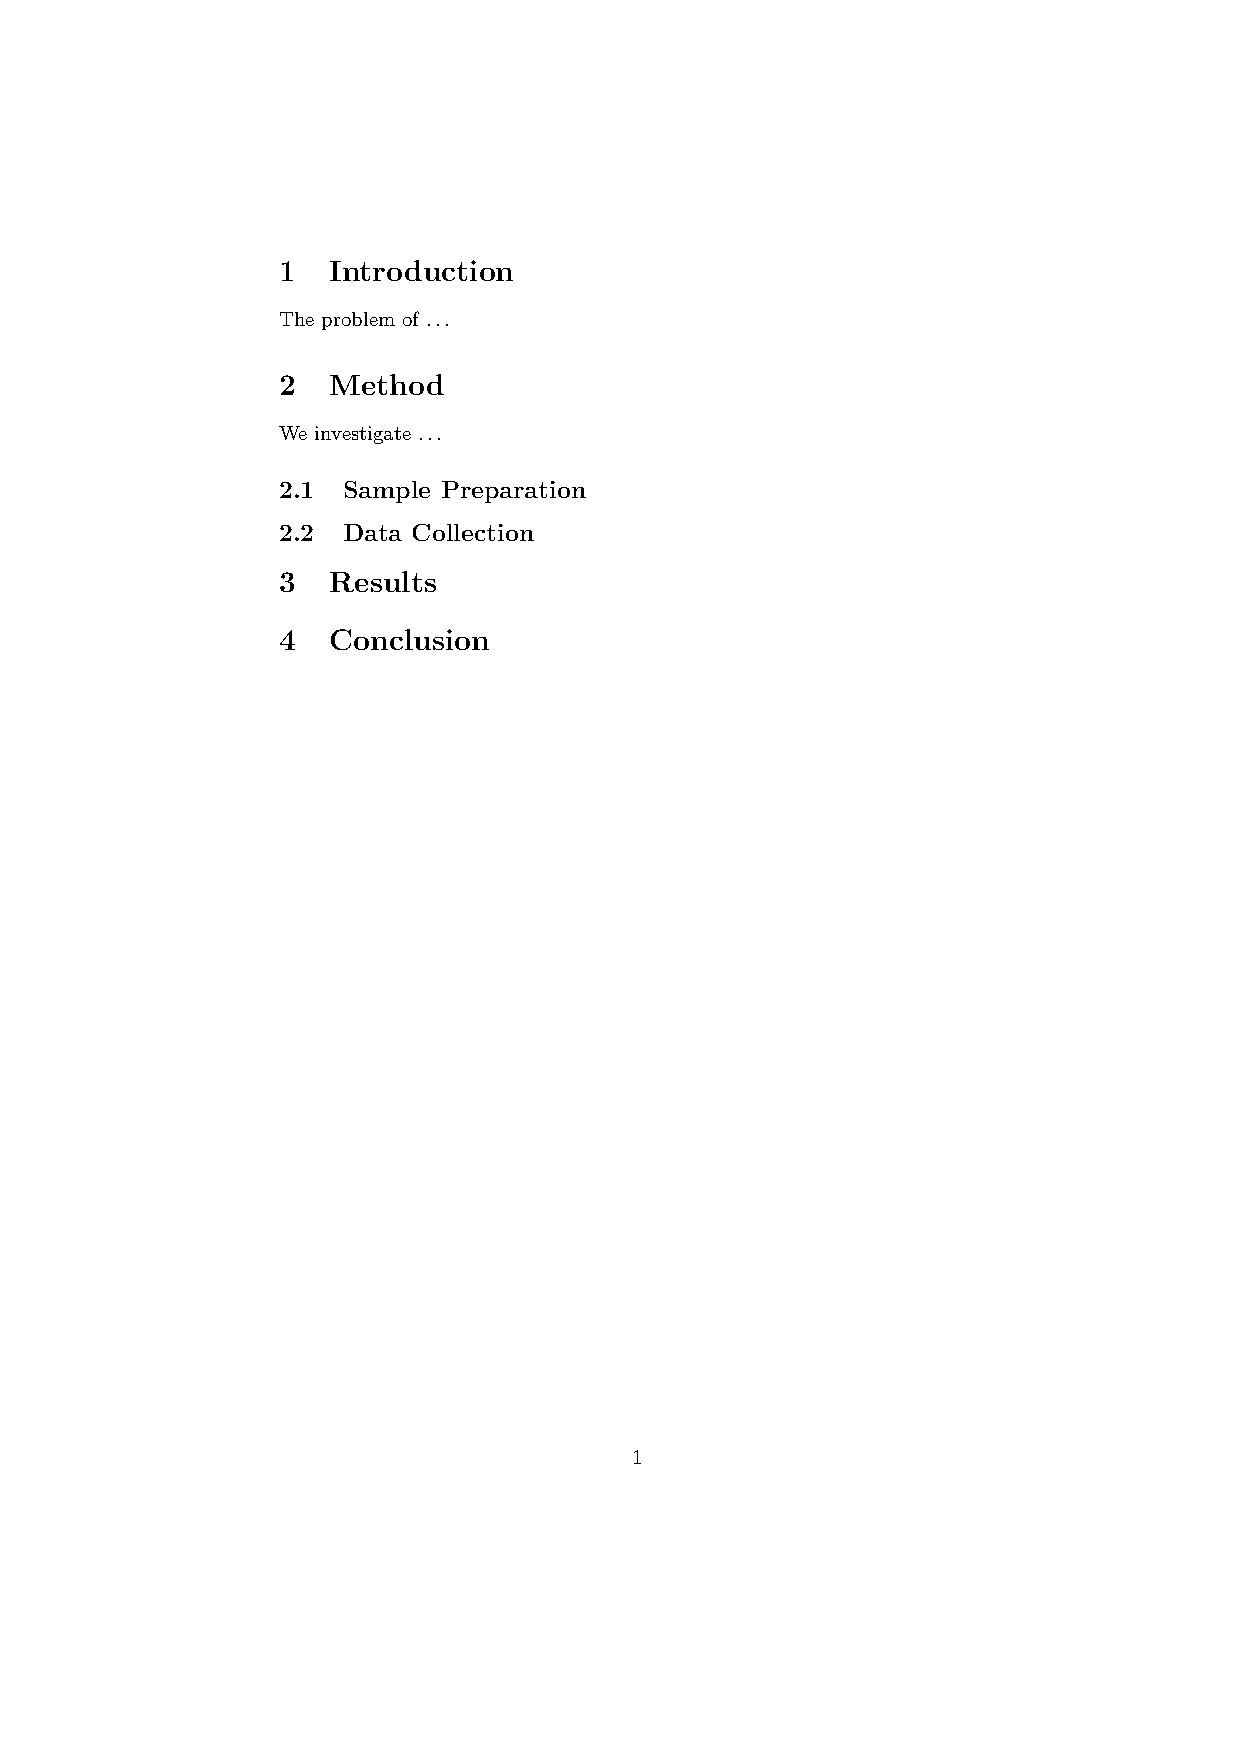
\includegraphics[width=\textwidth,clip,trim=1.5in 6in 4in 1in]{structure-sections.pdf}
\end{minipage}
\end{frame}

%%%%%%%%%%%%%%%%%%%%%%%%%%%%%%%%%%%%%%%%%%%%%%%%%%%%%%%%%%%%%%%%%%%%%%%%%%%%%%%
%%%%%%%%%%%%%%%%%%%%%%%%%%%%%%%%%%%%%%%%%%%%%%%%%%%%%%%%%%%%%%%%%%%%%%%%%%%%%%%
%%%%%%%%%%%%%%%%%%%%%%%%%%%%%%%%%%%%%%%%%%%%%%%%%%%%%%%%%%%%%%%%%%%%%%%%%%%%%%%
\subsection{Etichette e riferimenti incrociati}
\begin{frame}[fragile]{\insertsubsection}
\begin{itemize}{\small
\item Usate i comandi \cmdbs{label} e \cmdbs{ref} per la numerazione automatica
e i riferimenti incrociati.
\item Il pacchetto \bftt{amsmath} offre \cmdbs{eqref} per numerare
le equazioni.
\begin{itemize}
\item File \texttt{structure-crossref.tex}
\end{itemize}
}\end{itemize}
\begin{minipage}{0.50\linewidth}
\inputminted[fontsize=\scriptsize,frame=single,resetmargins]{latex}%
  {structure-crossref.tex}
\end{minipage}
\begin{minipage}{0.45\linewidth}
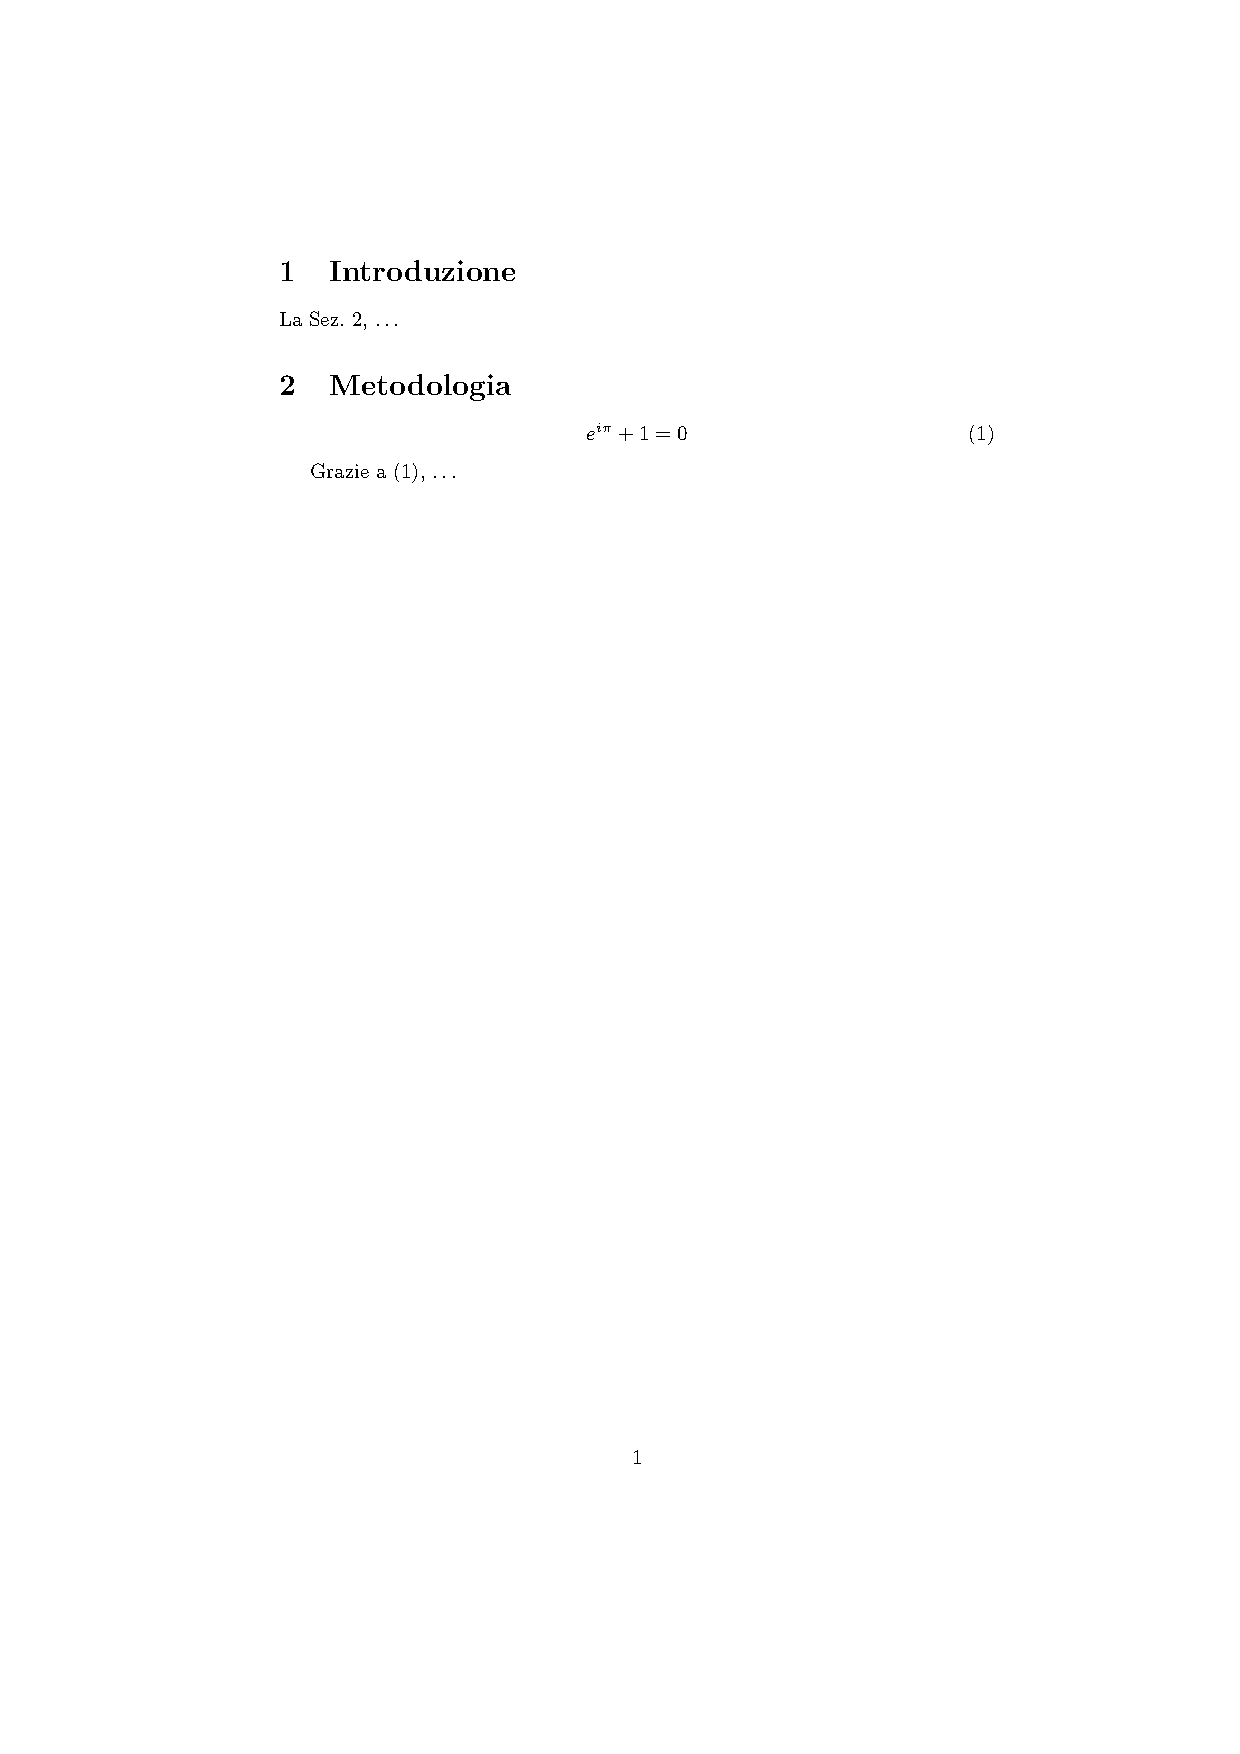
\includegraphics[width=\textwidth,clip,trim=1.5in 6in 1.6in 1in]{structure-crossref.pdf}
\end{minipage}
\end{frame}

%%%%%%%%%%%%%%%%%%%%%%%%%%%%%%%%%%%%%%%%%%%%%%%%%%%%%%%%%%%%%%%%%%%%%%%%%%%%%%%
%%%%%%%%%%%%%%%%%%%%%%%%%%%%%%%%%%%%%%%%%%%%%%%%%%%%%%%%%%%%%%%%%%%%%%%%%%%%%%%
%%%%%%%%%%%%%%%%%%%%%%%%%%%%%%%%%%%%%%%%%%%%%%%%%%%%%%%%%%%%%%%%%%%%%%%%%%%%%%%
\subsection{Esercizio}
\begin{frame}[fragile]{Esercizio sulla struttura dei documenti}

\begin{block}{Scrivi questo breve paper in \LaTeX\footnote{\url{http://pdos.csail.mit.edu/scigen/} --- un generatore casuale di paper.}:}
\begin{center}
\fbox{\href{\fileuri/structure-exercise-solution.pdf}{%
Clicca per aprire il paper (\texttt{structure-exercise-solution.pdf})}}
\end{center}
Cercate di rendere il paper simile a quello dell'esempio. Usate \cmdbs{ref} e \cmdbs{eqref} per evitare di scrivere esplicitamente nel testo i numeri
di sezione e delle equazioni.
\end{block}
\vskip 2ex
\begin{center}
\fbox{\href{\wlnewdoc{structure-exercise.tex}}{%
Clicca per aprire \texttt{structure-exercise.tex} con \wllogo{}}}
\end{center}

\begin{itemize}
\item Dopo qualche tentativo,
\fbox{\href{\wlnewdoc{structure-exercise-solution.tex}}{%
clicca qui per la mia soluzione}}.
\end{itemize}
\end{frame}

%%%%%%%%%%%%%%%%%%%%%%%%%%%%%%%%%%%%%%%%%%%%%%%%%%%%%%%%%%%%%%%%%%%%%%%%%%%%%%%
%%%%%%%%%%%%%%%%%%%%%%%%%%%%%%%%%%%%%%%%%%%%%%%%%%%%%%%%%%%%%%%%%%%%%%%%%%%%%%%
%%%%%%%%%%%%%%%%%%%%%%%%%%%%%%%%%%%%%%%%%%%%%%%%%%%%%%%%%%%%%%%%%%%%%%%%%%%%%%%
\section{Immagini e tabelle}

%%%%%%%%%%%%%%%%%%%%%%%%%%%%%%%%%%%%%%%%%%%%%%%%%%%%%%%%%%%%%%%%%%%%%%%%%%%%%%%
%%%%%%%%%%%%%%%%%%%%%%%%%%%%%%%%%%%%%%%%%%%%%%%%%%%%%%%%%%%%%%%%%%%%%%%%%%%%%%%
%%%%%%%%%%%%%%%%%%%%%%%%%%%%%%%%%%%%%%%%%%%%%%%%%%%%%%%%%%%%%%%%%%%%%%%%%%%%%%%
\begin{frame}{Indice}
\begin{multicols}{2}
\tableofcontents[currentsection]
\end{multicols}
\end{frame}

%%%%%%%%%%%%%%%%%%%%%%%%%%%%%%%%%%%%%%%%%%%%%%%%%%%%%%%%%%%%%%%%%%%%%%%%%%%%%%%
%%%%%%%%%%%%%%%%%%%%%%%%%%%%%%%%%%%%%%%%%%%%%%%%%%%%%%%%%%%%%%%%%%%%%%%%%%%%%%%
%%%%%%%%%%%%%%%%%%%%%%%%%%%%%%%%%%%%%%%%%%%%%%%%%%%%%%%%%%%%%%%%%%%%%%%%%%%%%%%
\subsection{Grafica}
\begin{frame}[fragile]{\insertsubsection}
\begin{itemize}
\item Per inserire immagini nel testo, serve il pacchetto \bftt{graphicx},
che offre il comando \cmdbs{includegraphics}.
\item I formati supportati per le immagini includono (solitamente)
JPEG, PNG e PDF. Altri pacchetti supportano altri formati.
\end{itemize}
\begin{exampletwouptiny}
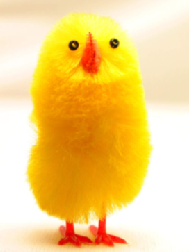
\includegraphics[
  width=0.5\textwidth]{pulcino_grande}

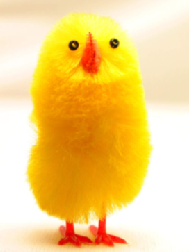
\includegraphics[
  width=0.3\textwidth,
  angle=270]{pulcino_grande}
\end{exampletwouptiny}

\tiny{Fonte: \url{http://www.andy-roberts.net/writing/latex/importing_images}}
\end{frame}

%%%%%%%%%%%%%%%%%%%%%%%%%%%%%%%%%%%%%%%%%%%%%%%%%%%%%%%%%%%%%%%%%%%%%%%%%%%%%%%
%%%%%%%%%%%%%%%%%%%%%%%%%%%%%%%%%%%%%%%%%%%%%%%%%%%%%%%%%%%%%%%%%%%%%%%%%%%%%%%
%%%%%%%%%%%%%%%%%%%%%%%%%%%%%%%%%%%%%%%%%%%%%%%%%%%%%%%%%%%%%%%%%%%%%%%%%%%%%%%
\begin{frame}[fragile]{Intermezzo: Argomenti Opzionali}
\begin{itemize}
\item Si usano le parentesi quadre \keystrokebftt{[} \keystrokebftt{]} per gli
argomenti opzionali, invece che le graffe \keystrokebftt{\{} \keystrokebftt{\}}.
\item \cmdbs{includegraphics} accetta una serie di opzioni che permettono di
trasformare l'immagine quando viene inclusa nel testo. Per esempio, \bftt{width=0.3\cmdbs{textwidth}} fa s\`i che l'immagine sia larga
quanto il 30\% del testo circostante\\(il cui valore \`e contenuto in \cmdbs{textwidth}).
\item Anche \cmdbs{documentclass} accetta opzioni. Per esempio:
\vskip 1.5ex
\mint{latex}|\documentclass[12pt,twocolumn]{article}|
\vskip 1.5ex
usa un font pi\`u grande di quello standard (12pt) e un layout a due colonne.
\item Come scoprire quali argomenti opzionali sono disponibili?
Alla fine della presentazione, mostrer\`o alcuni link\ldots
\end{itemize}
\end{frame}

%%%%%%%%%%%%%%%%%%%%%%%%%%%%%%%%%%%%%%%%%%%%%%%%%%%%%%%%%%%%%%%%%%%%%%%%%%%%%%%
%%%%%%%%%%%%%%%%%%%%%%%%%%%%%%%%%%%%%%%%%%%%%%%%%%%%%%%%%%%%%%%%%%%%%%%%%%%%%%%
%%%%%%%%%%%%%%%%%%%%%%%%%%%%%%%%%%%%%%%%%%%%%%%%%%%%%%%%%%%%%%%%%%%%%%%%%%%%%%%
\subsection[fragile]{Flottanti}
\begin{frame}{\insertsubsection}
\begin{itemize}
\item Permettono a \LaTeX{} di decidere il posizionamento della figura (potr\`a `flottare' -- o galleggiare -- nel testo).
\item Cos\`i facendo \`e anche possibile dare didascalie alle figure, che possono
essere richiamate con \cmdbs{ref}.
\begin{itemize}
\item File \texttt{media-graphics.tex}
\end{itemize}
\end{itemize}
\begin{minipage}{0.55\linewidth}
\inputminted[fontsize=\scriptsize,frame=single,resetmargins]{latex}%
  {media-graphics.tex}
\end{minipage}
\begin{minipage}{0.35\linewidth}
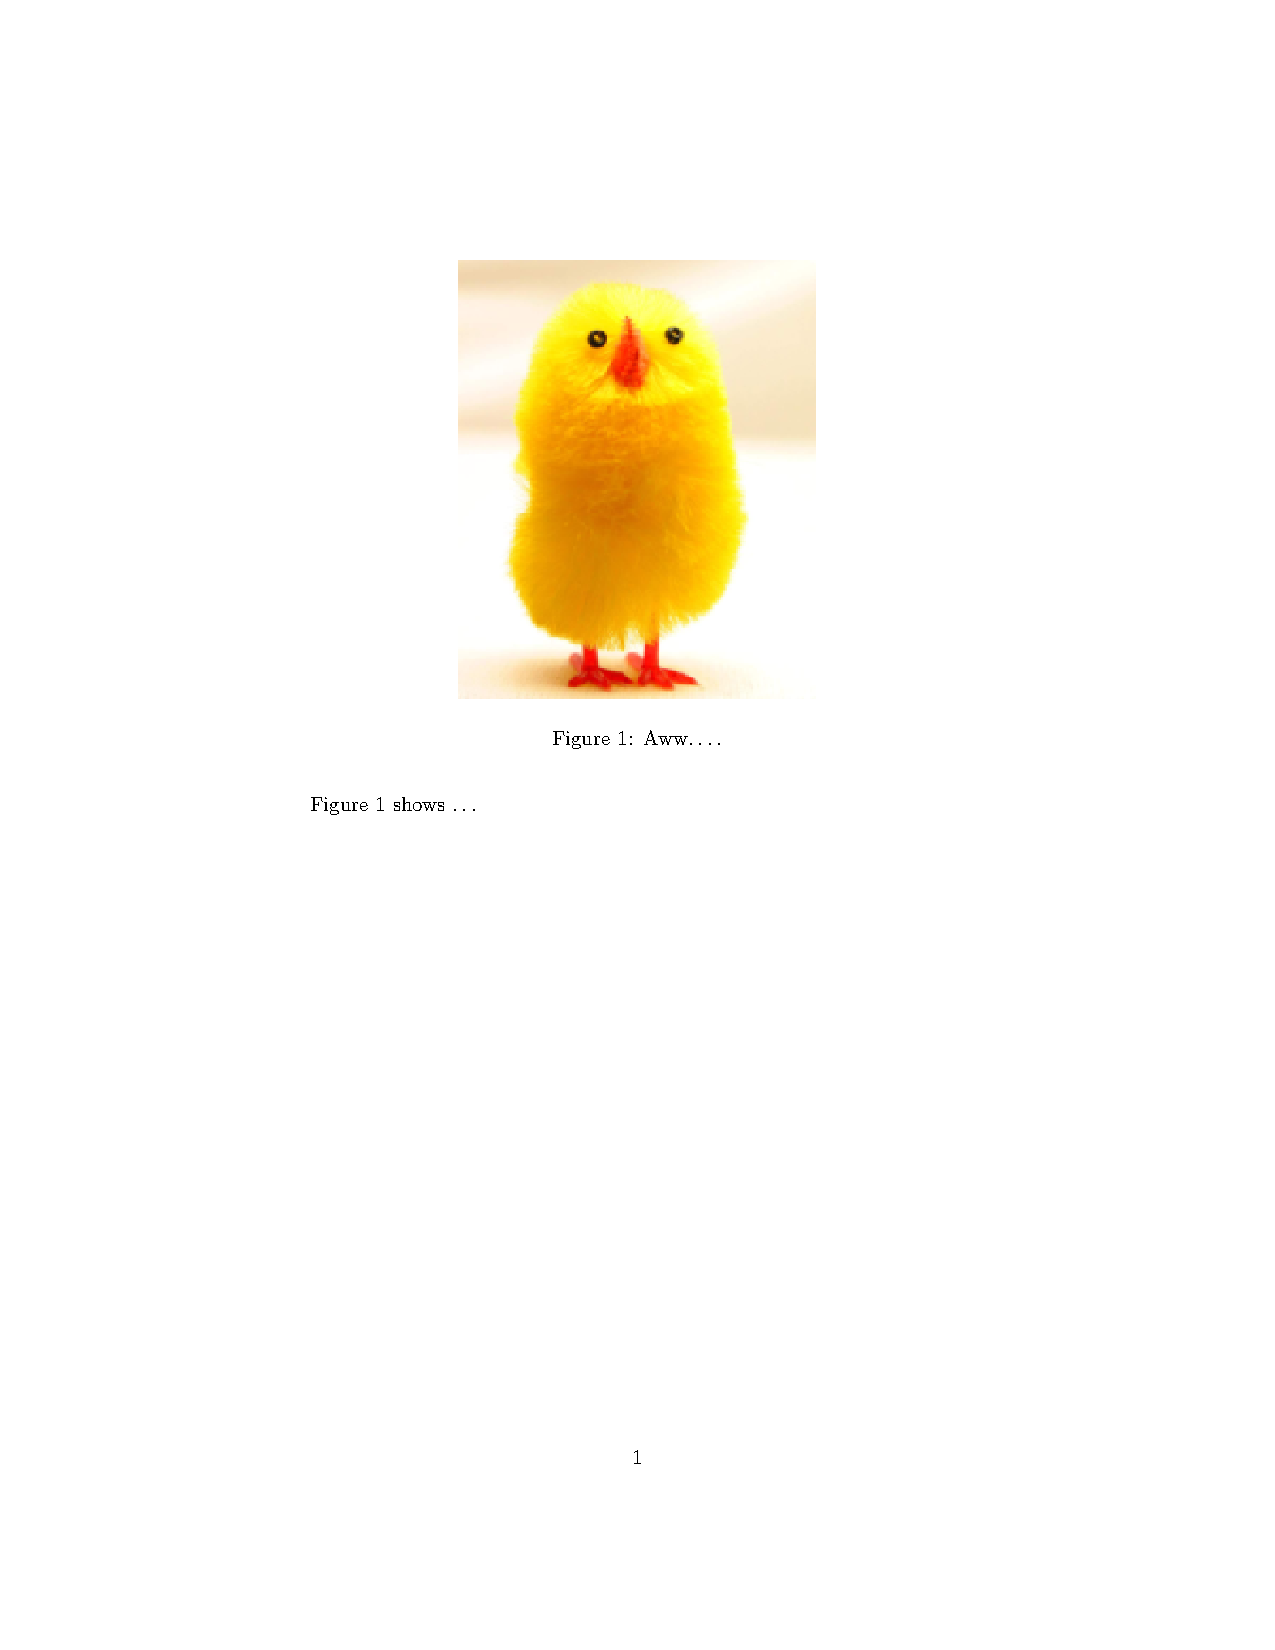
\includegraphics[width=\textwidth,clip,trim=2in 5in 3in 1in]{media-graphics.pdf}
\end{minipage}
\end{frame}

%%%%%%%%%%%%%%%%%%%%%%%%%%%%%%%%%%%%%%%%%%%%%%%%%%%%%%%%%%%%%%%%%%%%%%%%%%%%%%%
%%%%%%%%%%%%%%%%%%%%%%%%%%%%%%%%%%%%%%%%%%%%%%%%%%%%%%%%%%%%%%%%%%%%%%%%%%%%%%%
%%%%%%%%%%%%%%%%%%%%%%%%%%%%%%%%%%%%%%%%%%%%%%%%%%%%%%%%%%%%%%%%%%%%%%%%%%%%%%%
\subsection{Tabelle}
\begin{frame}[fragile]{\insertsubsection}
\begin{itemize}
\item Si usa l'ambiente \bftt{tabular} dal pacchetto \bftt{tabularx}.
\item L'argomento opzionale permette di impostare l'allineamento delle colonne --  \textbf{l}eft, \textbf{r}ight, \textbf{r}ight.
\begin{exampletwouptiny}
\begin{tabular}{lrr}
Art.   & Num & \euro \\
Tablet & 1   & 199.99  \\
PC     & 2   & 399.99  \\
Cavo   & 3   & 19.99   \\
\end{tabular}
\end{exampletwouptiny}
\item L'opzione \keystrokebftt{|} permette anche di specificare linee verticali;
per quelle orizzontali si usa \cmdbs{hline}.

\begin{exampletwouptiny}
\begin{tabular}{|l|r|r|} \hline
Art.   & Num & \euro   \\\hline
Tablet & 1   & 199.99  \\
PC     & 2   & 399.99  \\
Cavo   & 3   & 19.99   \\\hline
\end{tabular}
\end{exampletwouptiny}
\item Usa l'ampersand \keystrokebftt{\&} per separare le colonne e un doppio backslash \keystrokebftt{\bs}\keystrokebftt{\bs} per iniziare una nuova riga\\[0.5em]
\tiny come nell'ambiente \bftt{align*} che abbiamo visto nella Parte 1
\end{itemize}
\end{frame}

%%%%%%%%%%%%%%%%%%%%%%%%%%%%%%%%%%%%%%%%%%%%%%%%%%%%%%%%%%%%%%%%%%%%%%%%%%%%%%%
%%%%%%%%%%%%%%%%%%%%%%%%%%%%%%%%%%%%%%%%%%%%%%%%%%%%%%%%%%%%%%%%%%%%%%%%%%%%%%%
%%%%%%%%%%%%%%%%%%%%%%%%%%%%%%%%%%%%%%%%%%%%%%%%%%%%%%%%%%%%%%%%%%%%%%%%%%%%%%%
\addtocontents{toc}{\newpage}
\section{Bibliografia}

%%%%%%%%%%%%%%%%%%%%%%%%%%%%%%%%%%%%%%%%%%%%%%%%%%%%%%%%%%%%%%%%%%%%%%%%%%%%%%%
%%%%%%%%%%%%%%%%%%%%%%%%%%%%%%%%%%%%%%%%%%%%%%%%%%%%%%%%%%%%%%%%%%%%%%%%%%%%%%%
%%%%%%%%%%%%%%%%%%%%%%%%%%%%%%%%%%%%%%%%%%%%%%%%%%%%%%%%%%%%%%%%%%%%%%%%%%%%%%%
\begin{frame}{Indice}
\begin{multicols}{2}
\tableofcontents[currentsection]
\end{multicols}
\end{frame}

%%%%%%%%%%%%%%%%%%%%%%%%%%%%%%%%%%%%%%%%%%%%%%%%%%%%%%%%%%%%%%%%%%%%%%%%%%%%%%%
%%%%%%%%%%%%%%%%%%%%%%%%%%%%%%%%%%%%%%%%%%%%%%%%%%%%%%%%%%%%%%%%%%%%%%%%%%%%%%%
%%%%%%%%%%%%%%%%%%%%%%%%%%%%%%%%%%%%%%%%%%%%%%%%%%%%%%%%%%%%%%%%%%%%%%%%%%%%%%%
\subsection{bib\TeX}
\begin{frame}[fragile]{\insertsubsection{} 1}
\begin{itemize}
\item I riferimenti bibliografici andrebbero messi in un file \bftt{.bib}
usando il formato `bibtex' (es. \bftt{bib-example.bib}):

\inputminted[fontsize=\scriptsize,frame=single]{latex}{bib-example.bib}

\item La maggior parte dei motori di ricerca permettono di esportare
direttamente in formato bibtex
\end{itemize}
\end{frame}

%%%%%%%%%%%%%%%%%%%%%%%%%%%%%%%%%%%%%%%%%%%%%%%%%%%%%%%%%%%%%%%%%%%%%%%%%%%%%%%
%%%%%%%%%%%%%%%%%%%%%%%%%%%%%%%%%%%%%%%%%%%%%%%%%%%%%%%%%%%%%%%%%%%%%%%%%%%%%%%
%%%%%%%%%%%%%%%%%%%%%%%%%%%%%%%%%%%%%%%%%%%%%%%%%%%%%%%%%%%%%%%%%%%%%%%%%%%%%%%
\begin{frame}[fragile]{\insertsubsection{} 2}
\begin{itemize}
\item Ogni elemento in un file \bftt{.bib} ha una \structure{chiave} che si usa per farne riferimento nel testo.
\item Per esempio, \bftt{Scarson1999Stuff} \`e la chiave per l'articolo:

\begin{minted}[fontsize=\small,frame=single]{latex}
@Article{Scarson1999Stuff,
  author = {Von Scarson},
  ...
}
\end{minted}
\item Non \`e obbligatorio, ma una buona idea \`e di usare una chiave basata su
nome, anno e titolo del paper.
\item \LaTeX{} formatta in automatico le citazioni nel testo, e genera una bibliografia: sono disponibili tutti gli stili pi\`u comuni, e se ne possono generare di personalizzati.
\end{itemize}
\end{frame}

%%%%%%%%%%%%%%%%%%%%%%%%%%%%%%%%%%%%%%%%%%%%%%%%%%%%%%%%%%%%%%%%%%%%%%%%%%%%%%%
%%%%%%%%%%%%%%%%%%%%%%%%%%%%%%%%%%%%%%%%%%%%%%%%%%%%%%%%%%%%%%%%%%%%%%%%%%%%%%%
%%%%%%%%%%%%%%%%%%%%%%%%%%%%%%%%%%%%%%%%%%%%%%%%%%%%%%%%%%%%%%%%%%%%%%%%%%%%%%%
\begin{frame}[fragile]{\insertsubsection{} 3}
\begin{itemize}
\item Usate il pacchetto \bftt{natbib}\footnote{\bftt{biblatex}
\`e pi\`u ricco ma \bftt{natbib} \`e ancora il pi\`u diffuso e
usato in molti \emph{template} di riviste. File di esempio: \bftt{bib-example.tex}} con \cmdbs{citet} e \cmdbs{citep}.
\item Includete la bibliografia con il comando \cmdbs{bibliography} alla fine, e specificate uno stile con \cmdbs{bibliographystyle}.
\end{itemize}
\begin{minipage}{0.55\linewidth}
\inputminted[fontsize=\scriptsize,frame=single,resetmargins]{latex}%
  {bib-example.tex}
\end{minipage}
\begin{minipage}{0.35\linewidth}
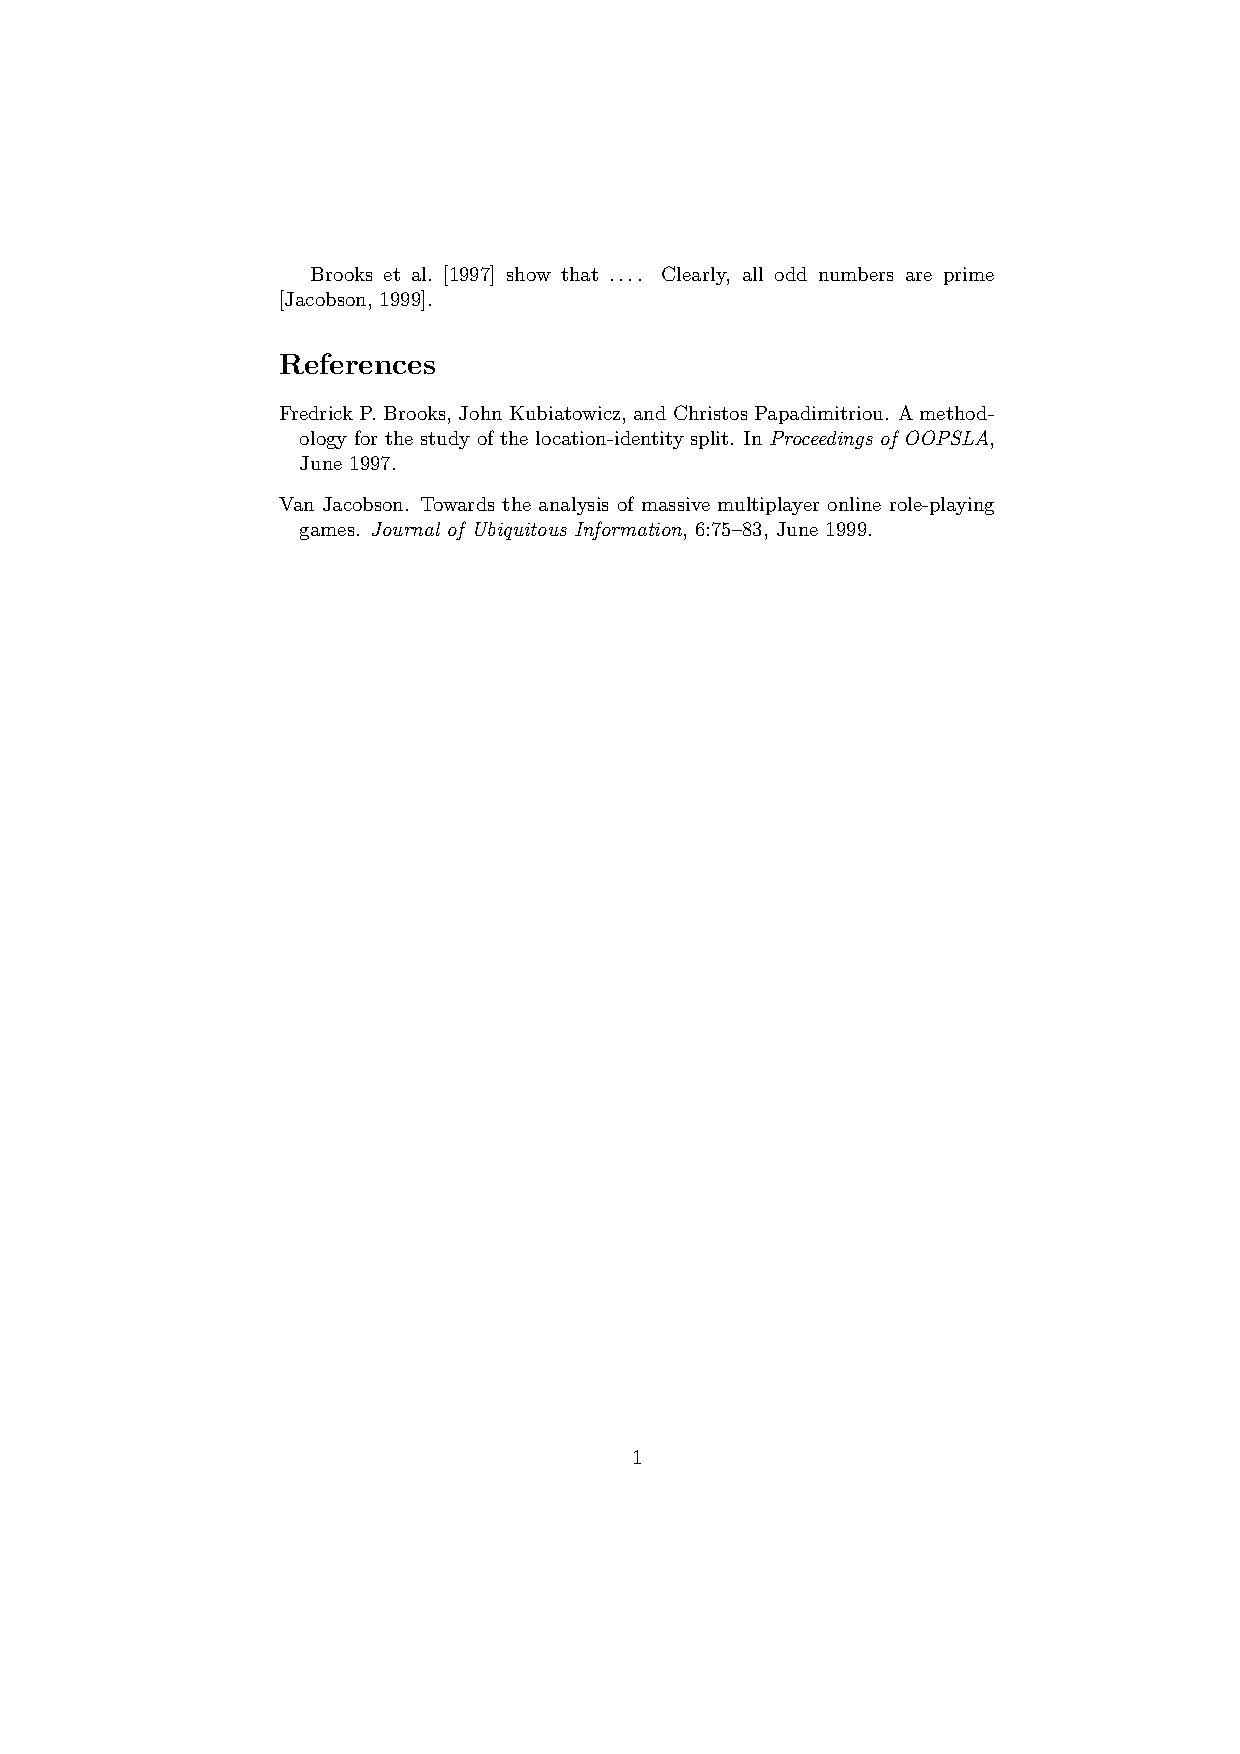
\includegraphics[width=\textwidth,clip,trim=1.8in 5in 1.8in 1in]{bib-example.pdf}
\end{minipage}
\end{frame}

%%%%%%%%%%%%%%%%%%%%%%%%%%%%%%%%%%%%%%%%%%%%%%%%%%%%%%%%%%%%%%%%%%%%%%%%%%%%%%%
%%%%%%%%%%%%%%%%%%%%%%%%%%%%%%%%%%%%%%%%%%%%%%%%%%%%%%%%%%%%%%%%%%%%%%%%%%%%%%%
%%%%%%%%%%%%%%%%%%%%%%%%%%%%%%%%%%%%%%%%%%%%%%%%%%%%%%%%%%%%%%%%%%%%%%%%%%%%%%%
\subsection{Esercizio}
\begin{frame}[fragile]{Esercizio: Mettiamo tutto insieme}

Provate ad aggiungere un'immagine e una bibliografia di esempio (generata casualmente) all'articolo dell'esercizio precedente.

\begin{enumerate}
\item Scarica questi file di esempio sul tuo computer.

\begin{center}
\fbox{\href{\fileuri/pulcino_grande.png?dl=1}
{Clicca per scaricare \bftt{pulcino\_grande.png}}}

\fbox{\href{\fileuri/bib-exercise.bib?dl=1}
{Clicca per scaricare \bftt{bib-exercise.bib}}}
\end{center}

\item Caricali su Overleaf (usa il men\`u \structure{Project}).

\end{enumerate}
\end{frame}

%%%%%%%%%%%%%%%%%%%%%%%%%%%%%%%%%%%%%%%%%%%%%%%%%%%%%%%%%%%%%%%%%%%%%%%%%%%%%%%
%%%%%%%%%%%%%%%%%%%%%%%%%%%%%%%%%%%%%%%%%%%%%%%%%%%%%%%%%%%%%%%%%%%%%%%%%%%%%%%
%%%%%%%%%%%%%%%%%%%%%%%%%%%%%%%%%%%%%%%%%%%%%%%%%%%%%%%%%%%%%%%%%%%%%%%%%%%%%%%
\section{E adesso?}

%%%%%%%%%%%%%%%%%%%%%%%%%%%%%%%%%%%%%%%%%%%%%%%%%%%%%%%%%%%%%%%%%%%%%%%%%%%%%%%
%%%%%%%%%%%%%%%%%%%%%%%%%%%%%%%%%%%%%%%%%%%%%%%%%%%%%%%%%%%%%%%%%%%%%%%%%%%%%%%
%%%%%%%%%%%%%%%%%%%%%%%%%%%%%%%%%%%%%%%%%%%%%%%%%%%%%%%%%%%%%%%%%%%%%%%%%%%%%%%
\begin{frame}{Indice}
\begin{multicols}{2}
\tableofcontents[currentsection]
\end{multicols}
\end{frame}

%%%%%%%%%%%%%%%%%%%%%%%%%%%%%%%%%%%%%%%%%%%%%%%%%%%%%%%%%%%%%%%%%%%%%%%%%%%%%%%
%%%%%%%%%%%%%%%%%%%%%%%%%%%%%%%%%%%%%%%%%%%%%%%%%%%%%%%%%%%%%%%%%%%%%%%%%%%%%%%
%%%%%%%%%%%%%%%%%%%%%%%%%%%%%%%%%%%%%%%%%%%%%%%%%%%%%%%%%%%%%%%%%%%%%%%%%%%%%%%
\subsection{\LaTeX{} intermedio\ldots}
\begin{frame}[fragile]{\insertsubsection}
\begin{itemize}
\item Aggiungi un indice con il comando \cmdbs{tableofcontents}
a partire dai comandi di sezionamento come \cmdbs{section}.

\item Cambia la classe del documento con \cmdbs{documentclass} a
\mint{latex}!\documentclass{scrartcl}!
o magari a
\mint{latex}!\documentclass[12pt]{IEEEtran}!

\item Definisci comandi personalizzati per un'equazione complessa:
\begin{exampletwouptiny}
\newcommand{\rperf}{%
  \rho_{\text{perf}}}
$$
\rperf = {\bf c}'{\bf X} + \varepsilon
$$
\end{exampletwouptiny}
\end{itemize}
\end{frame}

%%%%%%%%%%%%%%%%%%%%%%%%%%%%%%%%%%%%%%%%%%%%%%%%%%%%%%%%%%%%%%%%%%%%%%%%%%%%%%%
%%%%%%%%%%%%%%%%%%%%%%%%%%%%%%%%%%%%%%%%%%%%%%%%%%%%%%%%%%%%%%%%%%%%%%%%%%%%%%%
%%%%%%%%%%%%%%%%%%%%%%%%%%%%%%%%%%%%%%%%%%%%%%%%%%%%%%%%%%%%%%%%%%%%%%%%%%%%%%%
\subsection{Altri pacchetti\ldots}
\begin{frame}{\insertsubsection}
\begin{itemize}
\item \structure{\bftt{beamer}}: creazione di presentazioni (come questa!)
\item \structure{\bftt{todonotes}}: gestione commenti e TODO
\item \structure{\bftt{tikz}}: gestione della grafica
\item \structure{\bftt{pgfplots}}: per creare grafici in \LaTeX
\item \structure{\bftt{listings}}: per inserire codici sorgente nel testo
\item \structure{\bftt{spreadtab}}: creazione fogli di calcolo in \LaTeX{}
\item \structure{\bftt{gchords}}, \bftt{guitar}: spartiti e accordi per chitarra
\item \structure{\bftt{cwpuzzle}}: parole crociate
\end{itemize}
Vai su \url{https://www.overleaf.com/latex/examples} e \url{http://texample.net}
contengono numerosi esempi\ldots
\end{frame}

%%%%%%%%%%%%%%%%%%%%%%%%%%%%%%%%%%%%%%%%%%%%%%%%%%%%%%%%%%%%%%%%%%%%%%%%%%%%%%%
%%%%%%%%%%%%%%%%%%%%%%%%%%%%%%%%%%%%%%%%%%%%%%%%%%%%%%%%%%%%%%%%%%%%%%%%%%%%%%%
%%%%%%%%%%%%%%%%%%%%%%%%%%%%%%%%%%%%%%%%%%%%%%%%%%%%%%%%%%%%%%%%%%%%%%%%%%%%%%%
%\subsection{Installare \LaTeX{}}
%\begin{frame}{\insertsubsection}
%\begin{itemize}
%\item Per lavorare con \LaTeX{} sul vostro computer, e non su Overleaf, vi servir\`a una \structure{distribuzione}.
%\item Una distribuzione include il comando \bftt{latex} 
%e qualche migliaio di pacchetti.
%\begin{itemize}
%\item Su Windows: \href{http://miktex.org/}{Mik\TeX} o \href{http://tug.org/texlive/}{\TeX Live}
%\item Su Linux: \href{http://tug.org/texlive/}{\TeX Live}
%\item SU Mac: \href{http://tug.org/mactex/}{Mac\TeX}
%\end{itemize}
%\item Vi servir\`a anche un editor testuale con supporto \LaTeX{}. \small{\url{http://en.wikipedia.org/wiki/Comparison_of_TeX_editors}} compara tutte le possibili opzioni.
%\end{itemize}
%\end{frame}

%%%%%%%%%%%%%%%%%%%%%%%%%%%%%%%%%%%%%%%%%%%%%%%%%%%%%%%%%%%%%%%%%%%%%%%%%%%%%%%
%%%%%%%%%%%%%%%%%%%%%%%%%%%%%%%%%%%%%%%%%%%%%%%%%%%%%%%%%%%%%%%%%%%%%%%%%%%%%%%
%%%%%%%%%%%%%%%%%%%%%%%%%%%%%%%%%%%%%%%%%%%%%%%%%%%%%%%%%%%%%%%%%%%%%%%%%%%%%%%
\subsection{Risorse addizionali}
\begin{frame}{\insertsubsection}
\begin{itemize}
\item \structure{\href{http://en.wikibooks.org/wiki/LaTeX}{The \LaTeX{} Wikibook}} ---
materiale di riferimento e tutorial.
\item\structure{ \href{http://tex.stackexchange.com/}{\TeX{} Stack Exchange}} --- fai domande e ottieni risposte
\item \structure{\href{http://www.latex-community.org/}{\LaTeX{} Community}} --- il principale forum degli utilizzatori
\item \structure{\href{http://ctan.org/}{Comprehensive \TeX{} Archive Network (CTAN)}} ---
oltre quattromila pacchetti e relativa documentazione
\item Una ricerca diretta su \structure{Google}\ldots (che con tutta probabilit\`a vi porter\`a ad uno dei siti citati sopra)
\end{itemize}
\end{frame}

%%%%%%%%%%%%%%%%%%%%%%%%%%%%%%%%%%%%%%%%%%%%%%%%%%%%%%%%%%%%%%%%%%%%%%%%%%%%%%%
%%%%%%%%%%%%%%%%%%%%%%%%%%%%%%%%%%%%%%%%%%%%%%%%%%%%%%%%%%%%%%%%%%%%%%%%%%%%%%%
%%%%%%%%%%%%%%%%%%%%%%%%%%%%%%%%%%%%%%%%%%%%%%%%%%%%%%%%%%%%%%%%%%%%%%%%%%%%%%%
\begin{frame}
\begin{center}
Grazie dell'attenzione, e buon lavoro con \LaTeX{}!
\end{center}
\end{frame}

\end{document}

Contenuto addizionale:

Emphasized text is typed like this: \emph{this is emphasized}.
Bold       text is typed like this: \textbf{this is bold}.

Riferimenti:

--> maybe introduce the prettyref package here.

Tabelle:

Bonus points: check out the fp package and the spreadtab package.

Document Classes:

a .cls file (es. article) some journal templates come with one

-- For Typesetting Geeks

- dashes: -, --, ---
- ellipsis.
- controlling spaces: ~, \ , \,, \@
- spacing after periods (et al., etc.)
- Nested quotation marks: ``\,`

\begin{center}
\fbox{\href{http://ctan.org/}{The Comprehensive \TeX Archive Network (CTAN)}}
\end{center}